% Schematic of the angle rotation glue, in the plane normal to the
% junction curve.  Included by cpm_rotation_3d_results.tex.
%
% Convention: eta_t is the target branch's OUTWARD conormal, so the
% target branch itself lies along -eta_t.  The glue carries eta_s onto
% -eta_t, which is why the rotated node lands beside the target branch.
\begin{figure}[htbp]
\centering
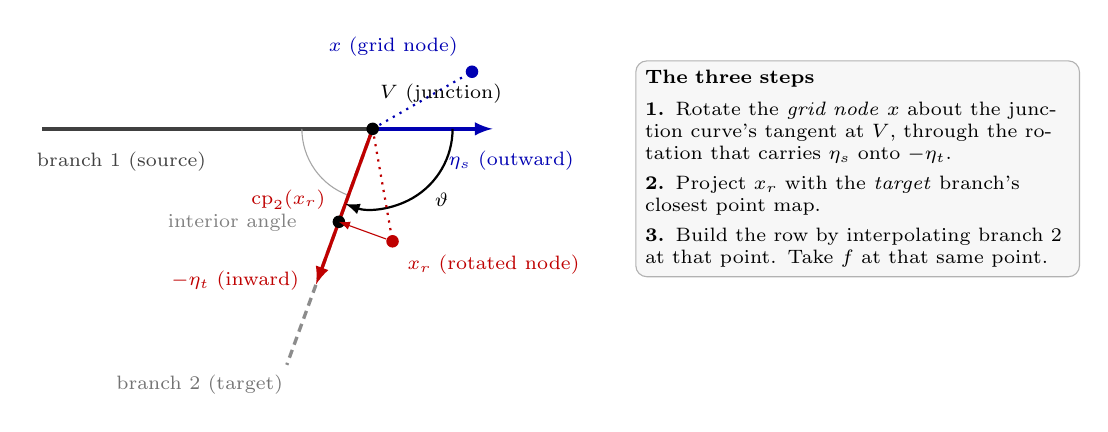
\begin{tikzpicture}[scale=1.45,>=latex,
    srcface/.style={very thick, black!75},
    tgtface/.style={very thick, black!45, densely dashed},
    node1/.style={circle, fill=blue!70!black, inner sep=1.6pt},
    node2/.style={circle, fill=red!75!black, inner sep=1.6pt},
    cp/.style={circle, fill=black, inner sep=1.6pt},
    lbl/.style={font=\scriptsize}]

  \coordinate (V) at (0,0);

  % ---- branch 1: the source face, along 180 degrees ----
  \draw[srcface] (V) -- (-2.90,0);
  \node[lbl, black!75, anchor=north] at (-2.20,-0.12)
      {branch 1 (source)};

  % ---- branch 2: the target face, along 250 degrees ----
  \draw[tgtface] (V) -- (-0.752,-2.067);
  \node[lbl, black!55, anchor=north east] at (-0.70,-2.07)
      {branch 2 (target)};

  % ---- the interior angle at the junction ----
  \draw[black!35] (-0.62,0) arc[start angle=180, end angle=250,
      radius=0.62];
  \node[lbl, black!50, anchor=north east] at (-0.58,-0.66)
      {interior angle};

  % ---- outward conormal of the source ----
  \draw[->, very thick, blue!70!black] (V) -- (1.05,0);
  \node[lbl, blue!70!black, anchor=north west] at (0.58,-0.11)
      {$\eta_s$ (outward)};

  % ---- inward direction of the target, along branch 2 ----
  \draw[->, very thick, red!75!black] (V) -- (-0.496,-1.363);
  \node[lbl, red!75!black, anchor=east] at (-0.56,-1.33)
      {$-\eta_t$ (inward)};

  % ---- the glue rotation ----
  \draw[->, thick, black] (0.70,0) arc[start angle=0,
      end angle=-110, radius=0.70];
  \node[lbl, anchor=west] at (0.46,-0.62) {$\vartheta$};

  % ---- the grid node, and its rotated image ----
  \node[node1] (X) at (0.87,0.50) {};
  \node[lbl, blue!70!black, anchor=south east] at (0.83,0.55)
      {$x$ (grid node)};
  \draw[blue!70!black, dotted, thick] (V) -- (X);

  \node[node2] (XR) at (0.174,-0.985) {};
  \node[lbl, red!75!black, anchor=north west] at (0.22,-1.02)
      {$x_r$ (rotated node)};
  \draw[red!75!black, dotted, thick] (V) -- (XR);

  % ---- the closest point of the rotated node on branch 2 ----
  \coordinate (CPT) at (-0.296,-0.814);
  \node[cp] at (CPT) {};
  \draw[->, red!75!black, thin] (XR) -- (CPT);
  \node[lbl, red!75!black, anchor=south east] at (-0.33,-0.79)
      {$\mathrm{cp}_2(x_r)$};

  \node[cp] at (V) {};
  \node[lbl, anchor=south west] at (-0.02,0.14) {$V$ (junction)};

  % ---- annotation box, clear of the drawing ----
  \node[draw=black!30, fill=black!3, rounded corners, align=left,
        lbl, text width=5.4cm, anchor=north west] at (2.30,0.60)
      {\textbf{The three steps}\\[1.2mm]
       \textbf{1.} Rotate the \emph{grid node} $x$ about the junction
          curve's tangent at $V$, through the rotation that carries
          $\eta_s$ onto $-\eta_t$.\\[1mm]
       \textbf{2.} Project $x_r$ with the \emph{target} branch's
          closest point map.\\[1mm]
       \textbf{3.} Build the row by interpolating branch 2 at that
          point. Take $f$ at that same point.};

\end{tikzpicture}
\caption{The angle rotation glue, drawn in the plane normal to the
  junction curve. Here $\eta_t$ is the target branch's \emph{outward}
  conormal, so branch 2 itself lies along $-\eta_t$. The rotation carries
  the source branch's outward direction $\eta_s$ onto $-\eta_t$. Leaving
  one branch means entering the other, so outward-onto-inward is the
  pairing a rigid continuation needs. The object that is rotated is the
  grid node $x$, not its closest point. This carries both the overhang
  past the junction and the normal offset across intact. On the ellipsoid
  this plane is a meridian half plane, and one angle serves the whole cut
  circle. On the tube the plane is the normal plane of a corner curve,
  and the angle varies along the curve, because the twist stops the two
  faces from being perpendicular.}
\label{fig:glue}
\end{figure}
